\providecommand{\main}{../../..}
\documentclass[\main/dresen_thesis.tex]{subfiles}

\begin{document}
  \section{Small-Angle X-ray Scattering (SAXS)}
    \label{ch:methods:saxs}
    In SAXS experiments as presented in this work, a X-ray beam with small spot size is directed on nanoparticles in dispersion, which are filled into capillaries, and the scattered intensity is recorded on a position-sensitive detector at a sample-to-detector distance $L_\mathrm{SDD}$ behind the sample.
    The used capillaries are made of borosilicate glass and have a diameter of $d \approx 1.5\unit{mm}$ to minimize multiple scattering events in the dispersion.
    They are sealed with a small plastic stopper and a glue gun to allow the measurement of the dispersions in a vacuum.
    All SAXS measurements in this thesis are performed on the GALAXI instrument (\refsec{ch:lss:galaxi}).
    To measure multiple samples over the course of a day automatically within the same setup, the capillaries are placed in a sample holder that can hold up to 11 capillaries, which is shown in \reffig{fig:methods:saxs:samples}.
    The sample holder can be shifted vertically to bring the respective capillary of the dispersion of interest into the beam path.
    \begin{figure}[tb]
      \centering
      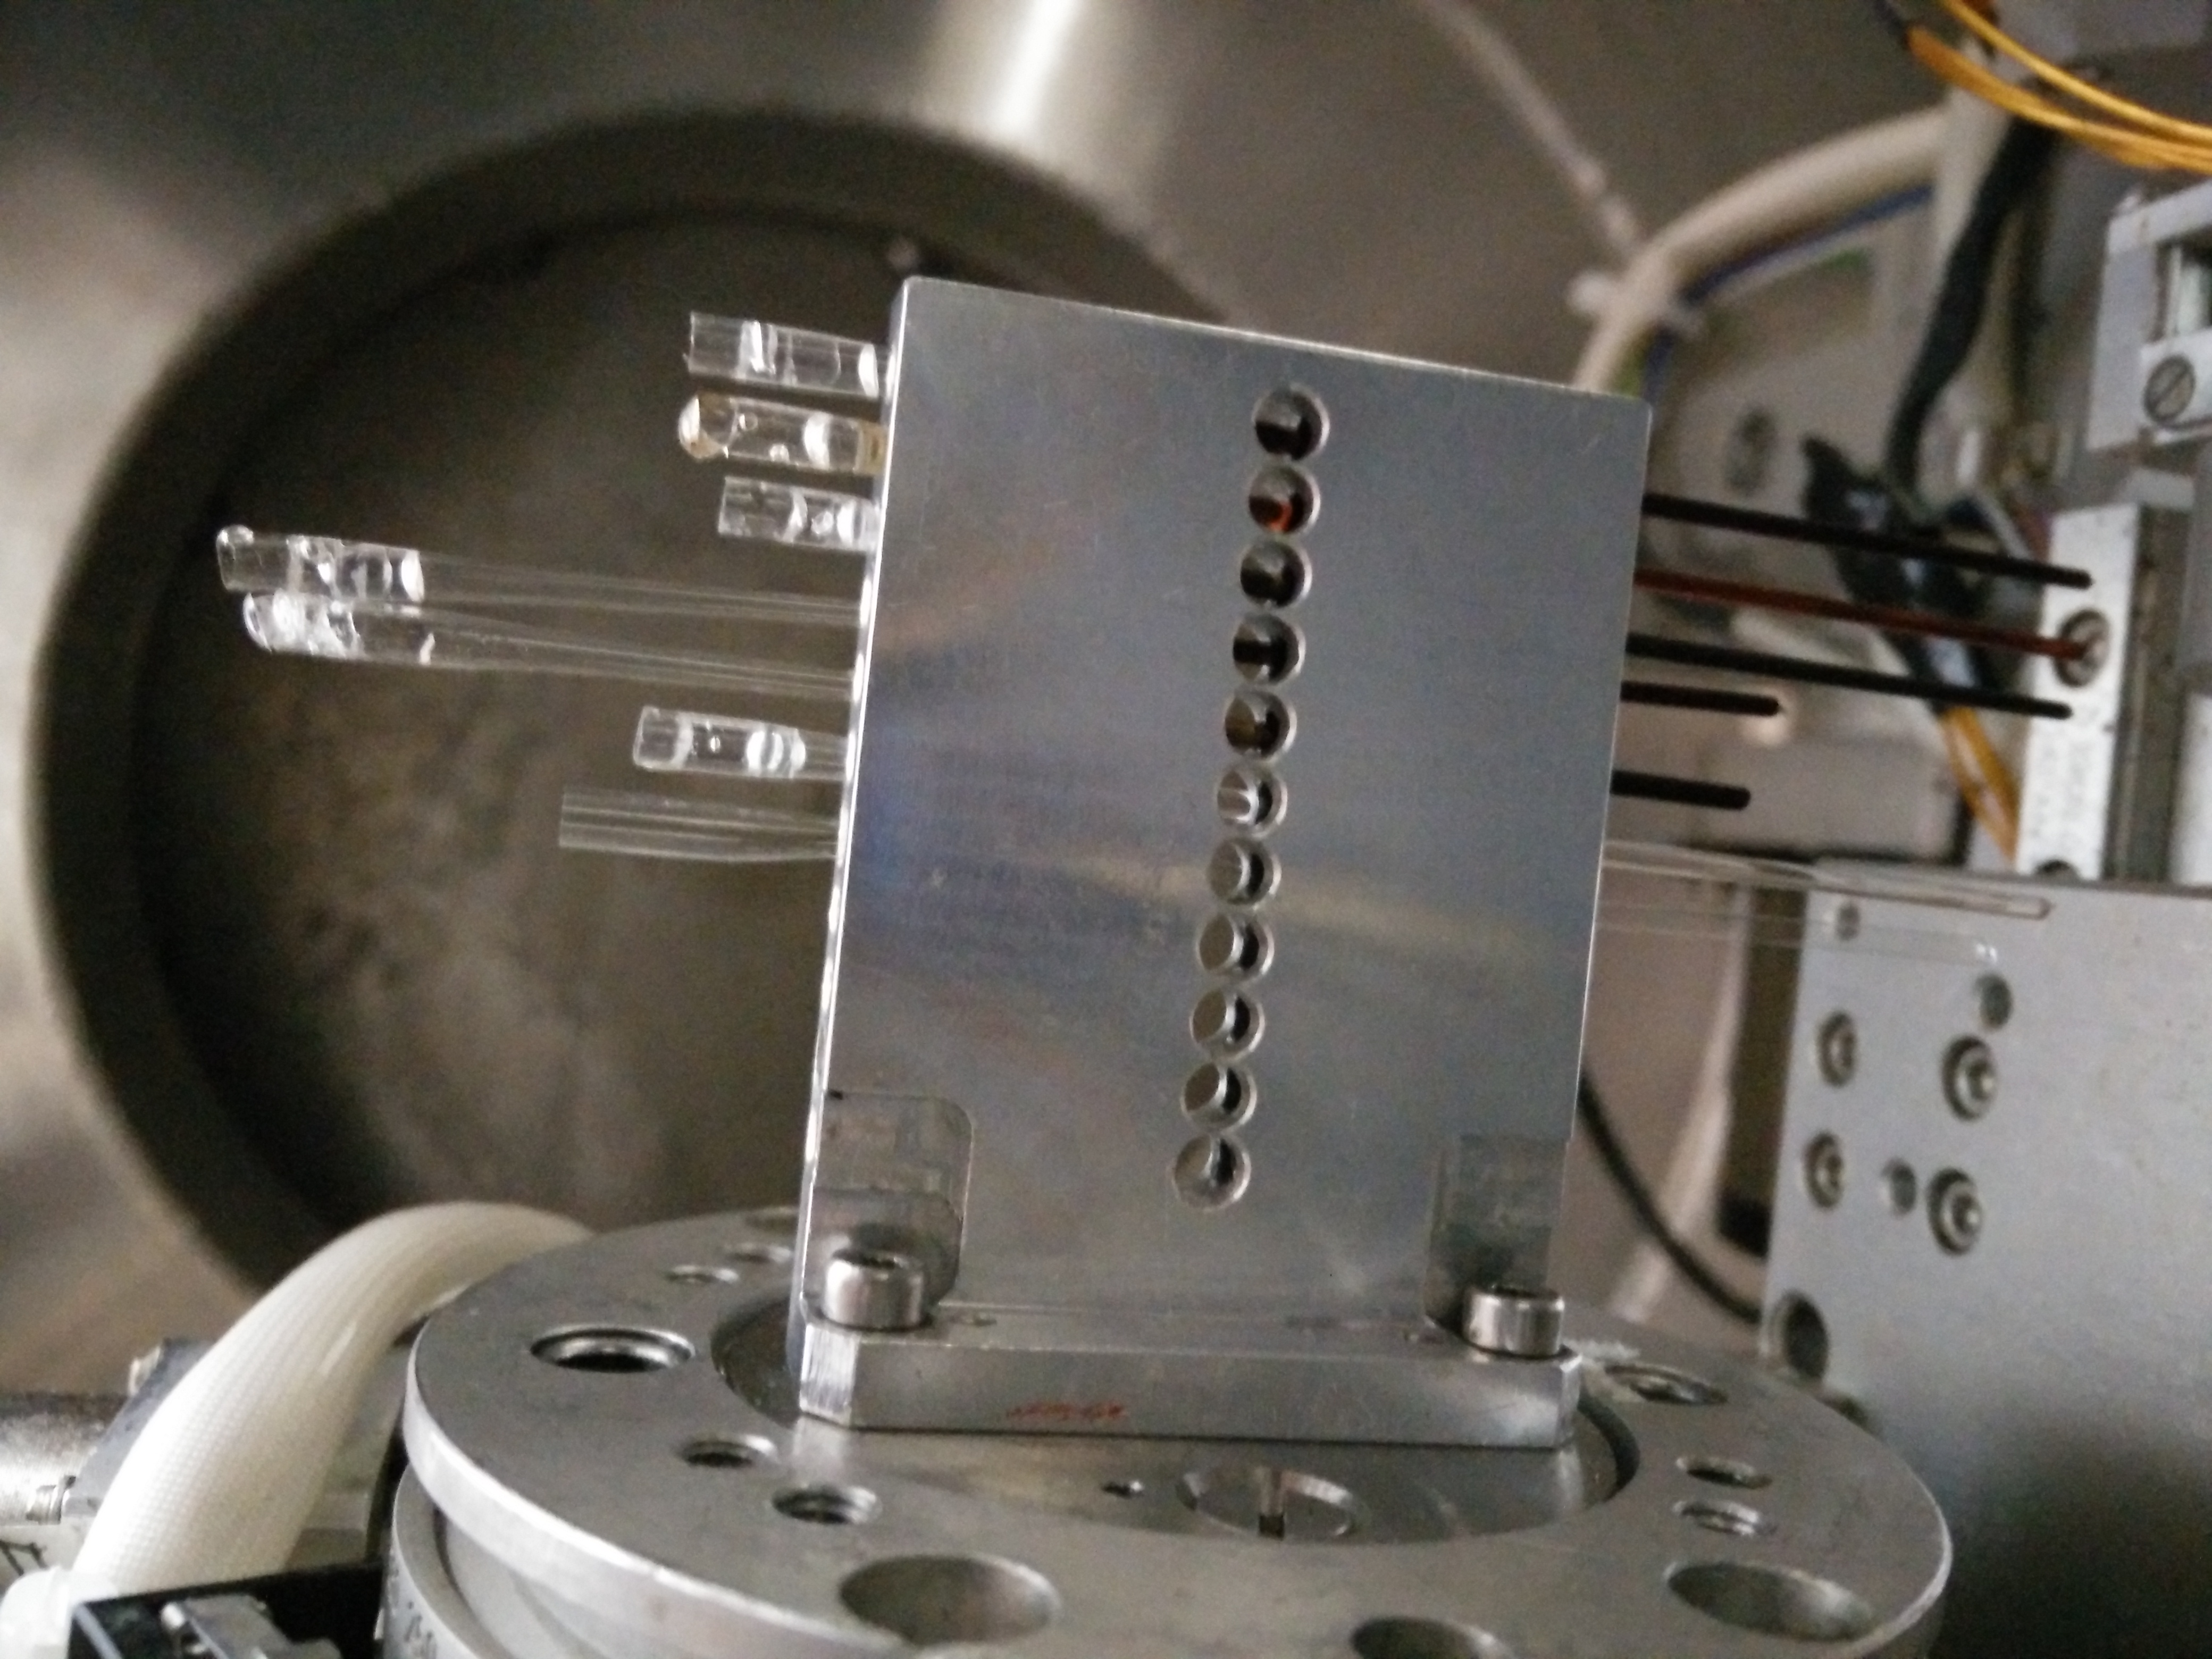
\includegraphics[width=0.7\textwidth]{appendix_methods_saxs_samples}
      \caption{\label{fig:methods:saxs:samples} SAXS samples stacked in a sample holder that can be moved in vertical direction for automatized measurement of multiple dispersions over a day. }
    \end{figure}

    To determine the beam center position and the distance $L_\mathrm{SDD}$ during an experiment, a piece of silver behenate (AgBH) is measured for a short time of $120 \unit{s}$.
    AgBH produces sharp rings at multiples of a scattering vector with magnitude $q_\mathrm{AgBH} \eq 1.076 \unit{\nm^{-1}}$.
    Thus, by doing the azimuthal integration of the detector data, as shown in \reffig{fig:methods:saxs:agBH}, both the beam center and the sample-to-detector distance can be determined quickly.
    If the estimate of the pixel position of the beam center is slightly off, the transformation to polar coordinates does not produce horizontal, but bended lines, which results in broadened peaks in the azimuthal integration.
    By varying the beam center position around an initial guess that is read from the detector image, the best value can be determined by searching for the center position that minimizes the peak width in the azimuthal integration.
    The distance $L_\mathrm{SDD}$ is obtained by determining, whether the peak center positions are truly at multiples of $q_\mathrm{AgBH}$.
    To load the raw data files obtained from the detector, the Python package FabIO \cite{Knudsen_2013_Fabio} is used and for the coordinate transformation / azimuthal integration, the package pyFAI is leveraged \cite{Ashiotis_2015_Thefa}.
    \begin{figure}[tb]
      \centering
      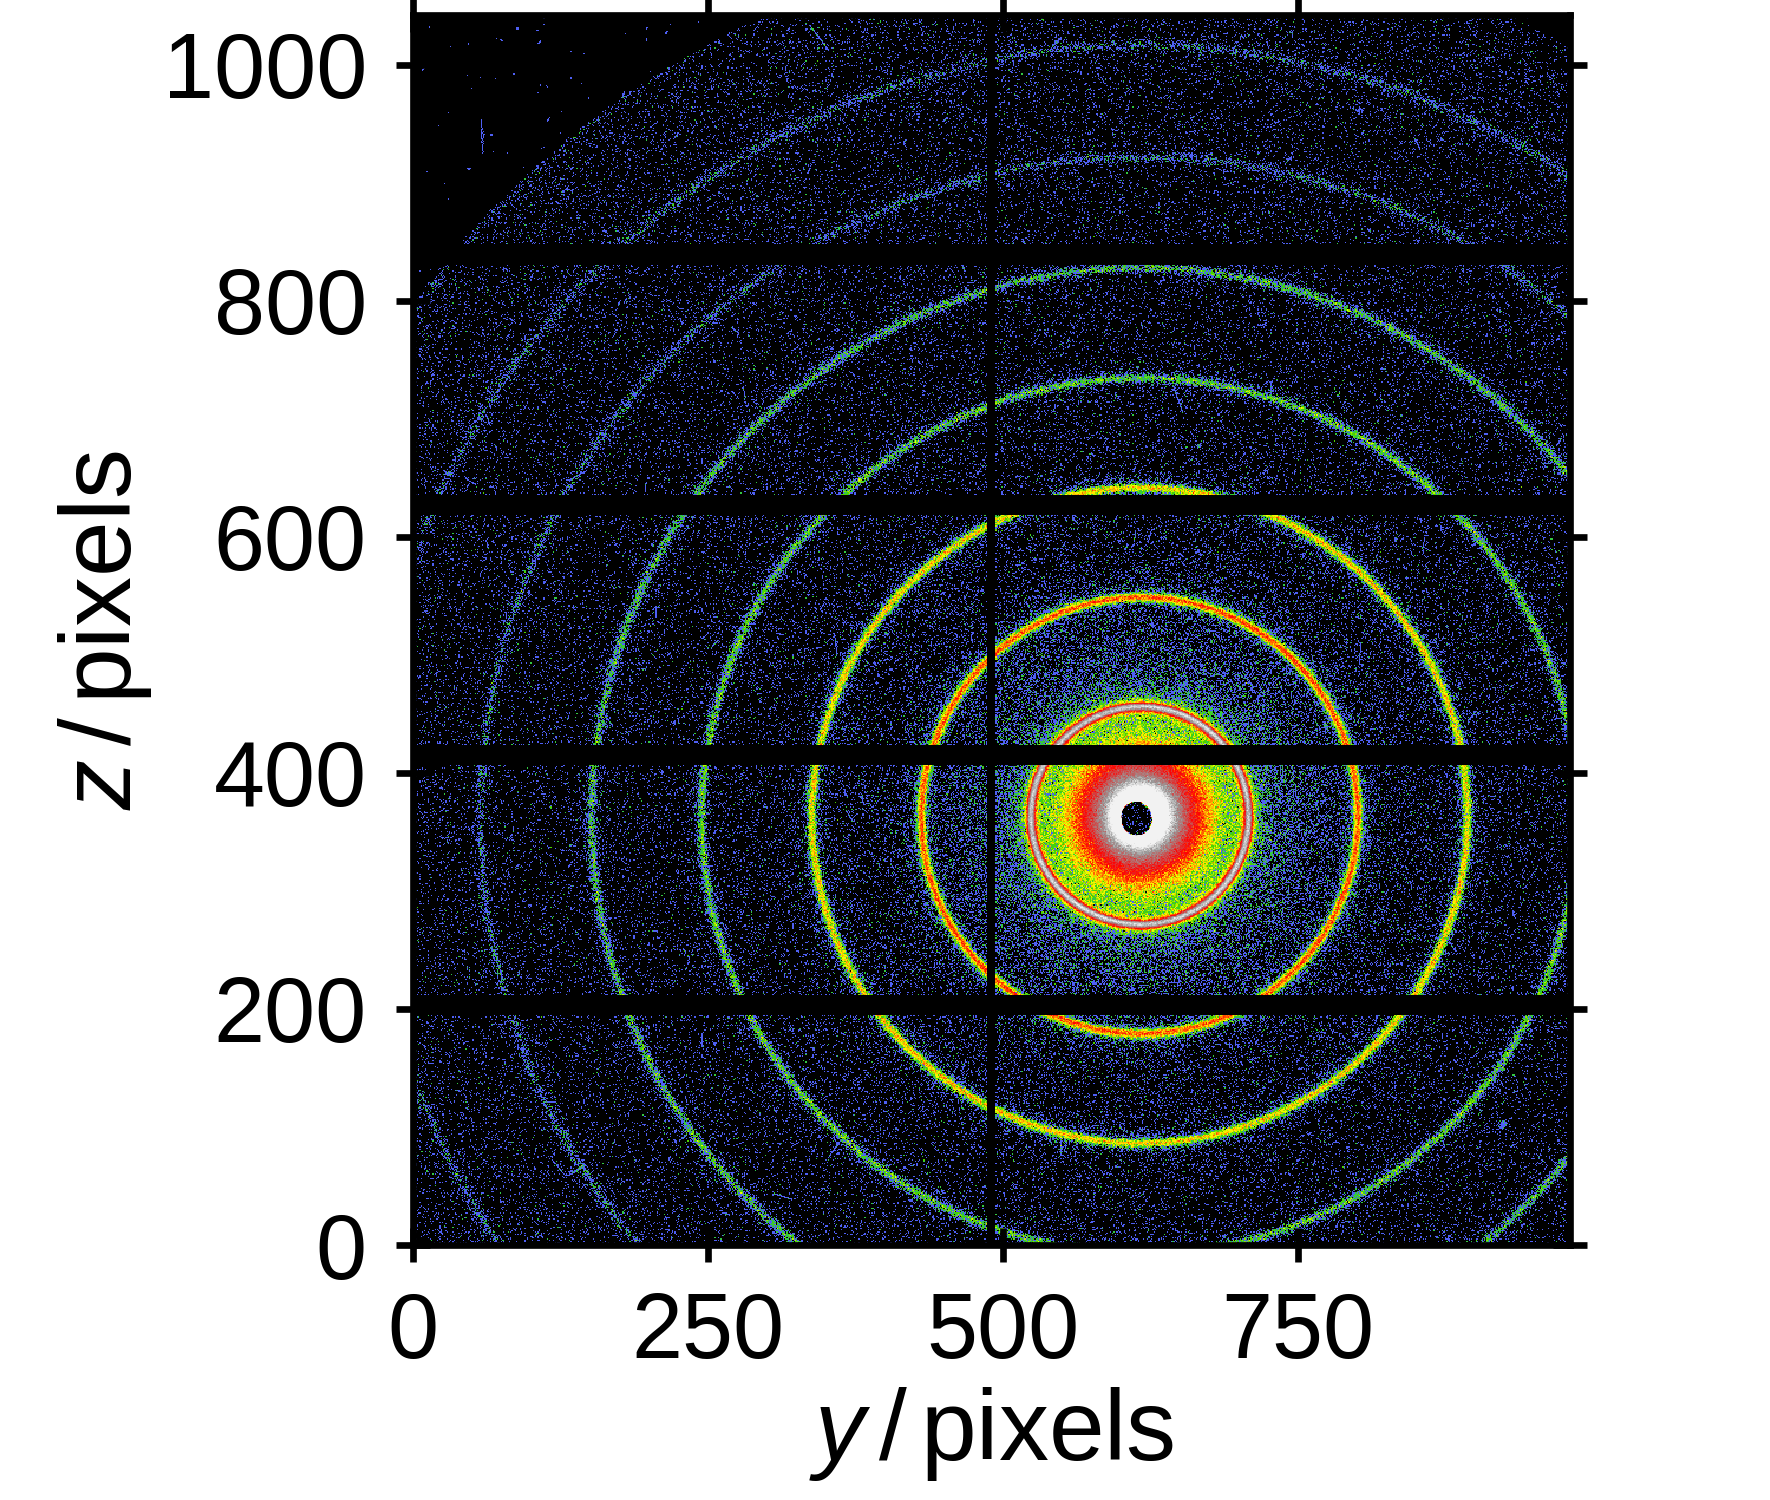
\includegraphics{appendix_methods_SAXS_AgBH}
      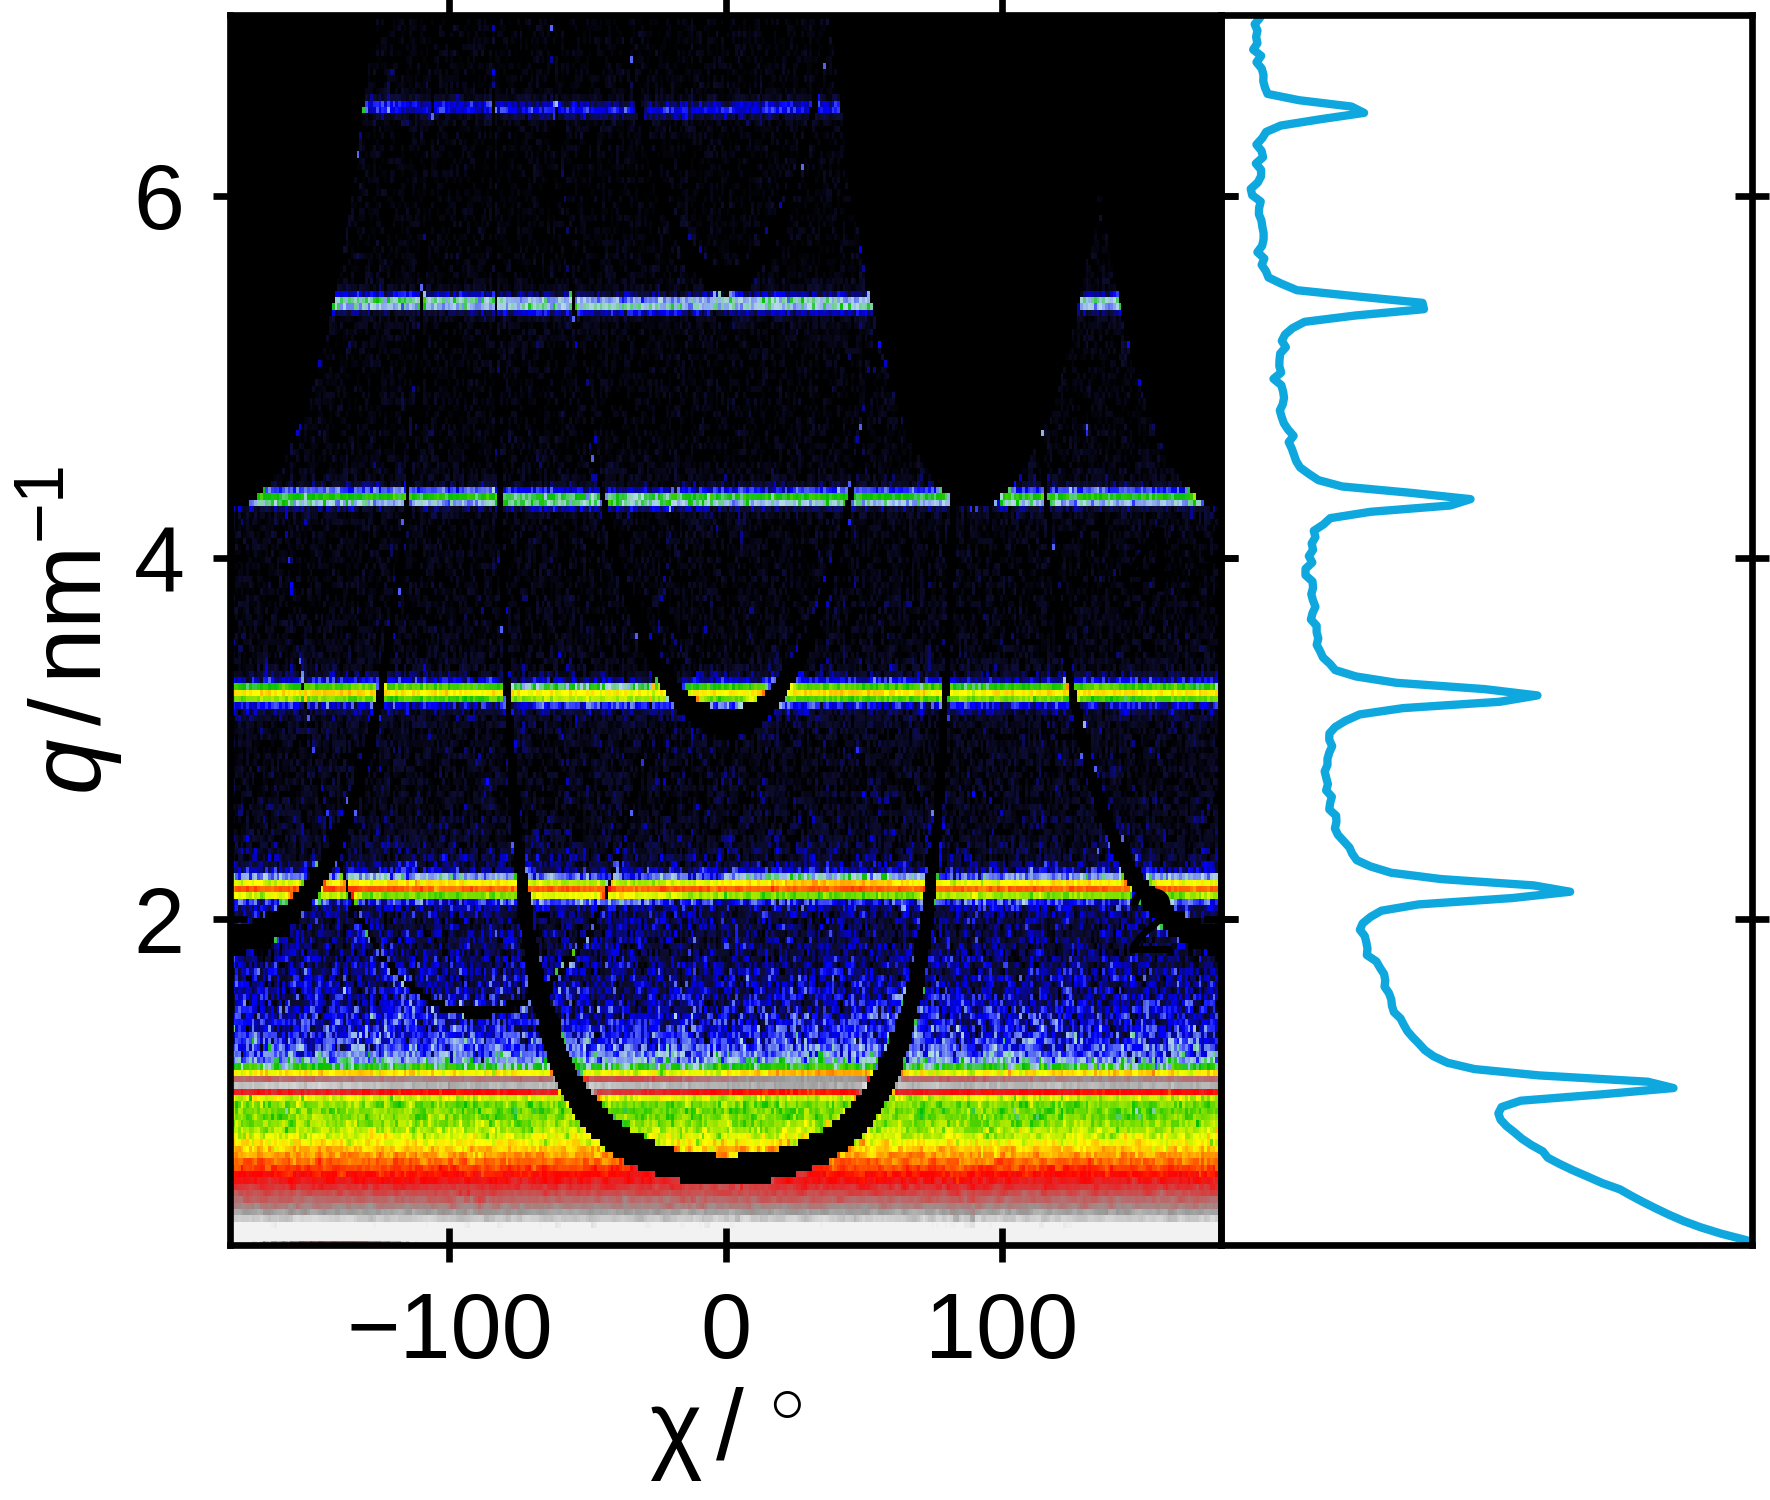
\includegraphics{appendix_methods_SAXS_AgBH_azimuthal}
      \caption{\label{fig:methods:saxs:agBH}AgBH calibration measurement to determine the beam center position and sample-to-detector distance. The measured intensity on the detector (left) is transformed to polar coordinates (right), where from the projection on $q$ the optimal parameters for beam position and distance are determined.}
    \end{figure}

    To put the arbitrary count rate of the position-sensitive detector into absolute units of $\unit{cm^{-1}}$, a pre-characterized calibration sample needs to be measured to determine the conversion factor.
    For the samples measured at the GALAXI instrument (\refsec{ch:lss:galaxi}), a piece of fluorinated ethylene propylene (FEP) is measured at the largest possible distance before every experiment, which produces a broad ring on the detector where the peak value $I_\mathrm{FEP}^\mathrm{peak}$ is compared to a measurement of FEP that was performed at an ESRF beam line \cite{Meyer_2009_Struk}.
    Furthermore for the scaling of the intensity, parameters specific to the measurement of the sample need to be considered.
    A different sample-to-detector distance $L_\mathrm{SDD}$ for sample and FEP measurement needs to be accounted, as the counting rate drops with the square of the distance.
    Also the transmission $T$ and thickness $d$ change from FEP to the sample needs to be included in the rescaling.
    Including all factors in one rescaling factor, it is given by
    \begin{align}
      \mathrm{scale factor} \eq \frac{1.212}{I_\mathrm{FEP}^\mathrm{peak} T_\mathrm{s} d_\mathrm{s}} \frac{c^\mathrm{monitor}_\mathrm{FEP}}{c_\mathrm{s}^\mathrm{monitor}} \frac{L^2_\mathrm{SSD,\, s}}{L^2_\mathrm{SSD, FEP}},
    \end{align}
    where the numeric value is the product of the ESRF measurement of FEP ($\dint \Sigma / \dint \Omega_\mathrm{FEP}^\mathrm{peak} \eq 0.6657(2) \unit{cm}^{-1}$), the transmission of FEP at the wavelength of GALAXI ($T_\mathrm{FEP} \eq 0.52$) and the thickness of the FEP sample ($d_\mathrm{FEP} \eq 0.035 \unit{cm}$).
    The sample transmission, thickness, monitor value and sample-to-detector distance are marked with $s$ in the index.

    The thickness and transmission of the sample, which are included in the rescaling factor, are determined by scanning over the vertical profile of the sample and measuring the intensity of the beam on a single-pixel detector.
    \begin{figure}[tb]
      \centering
      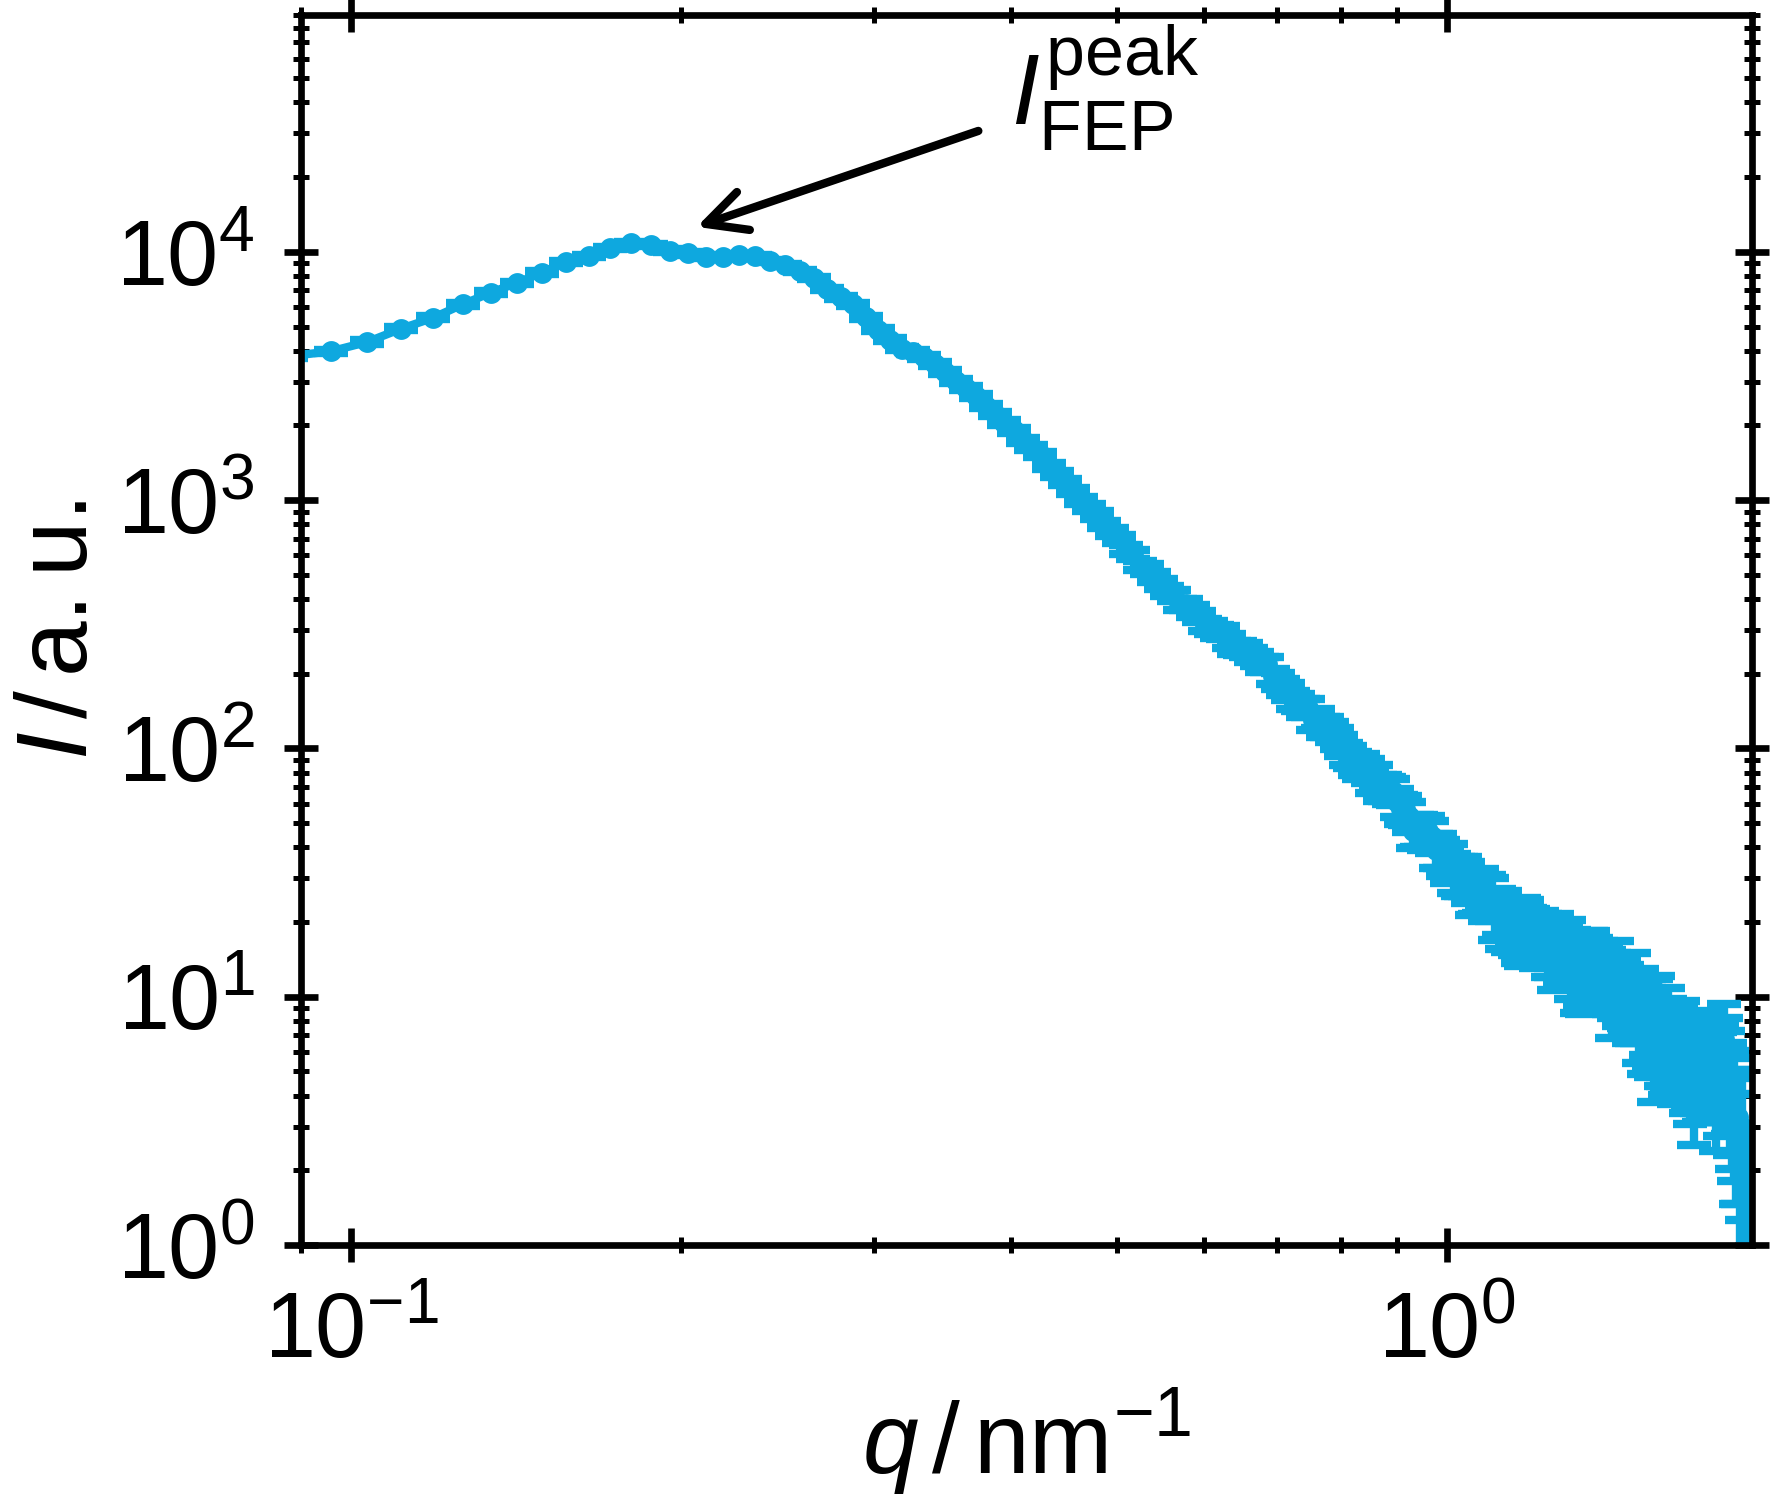
\includegraphics{appendix_methods_SAXS_FEP}
      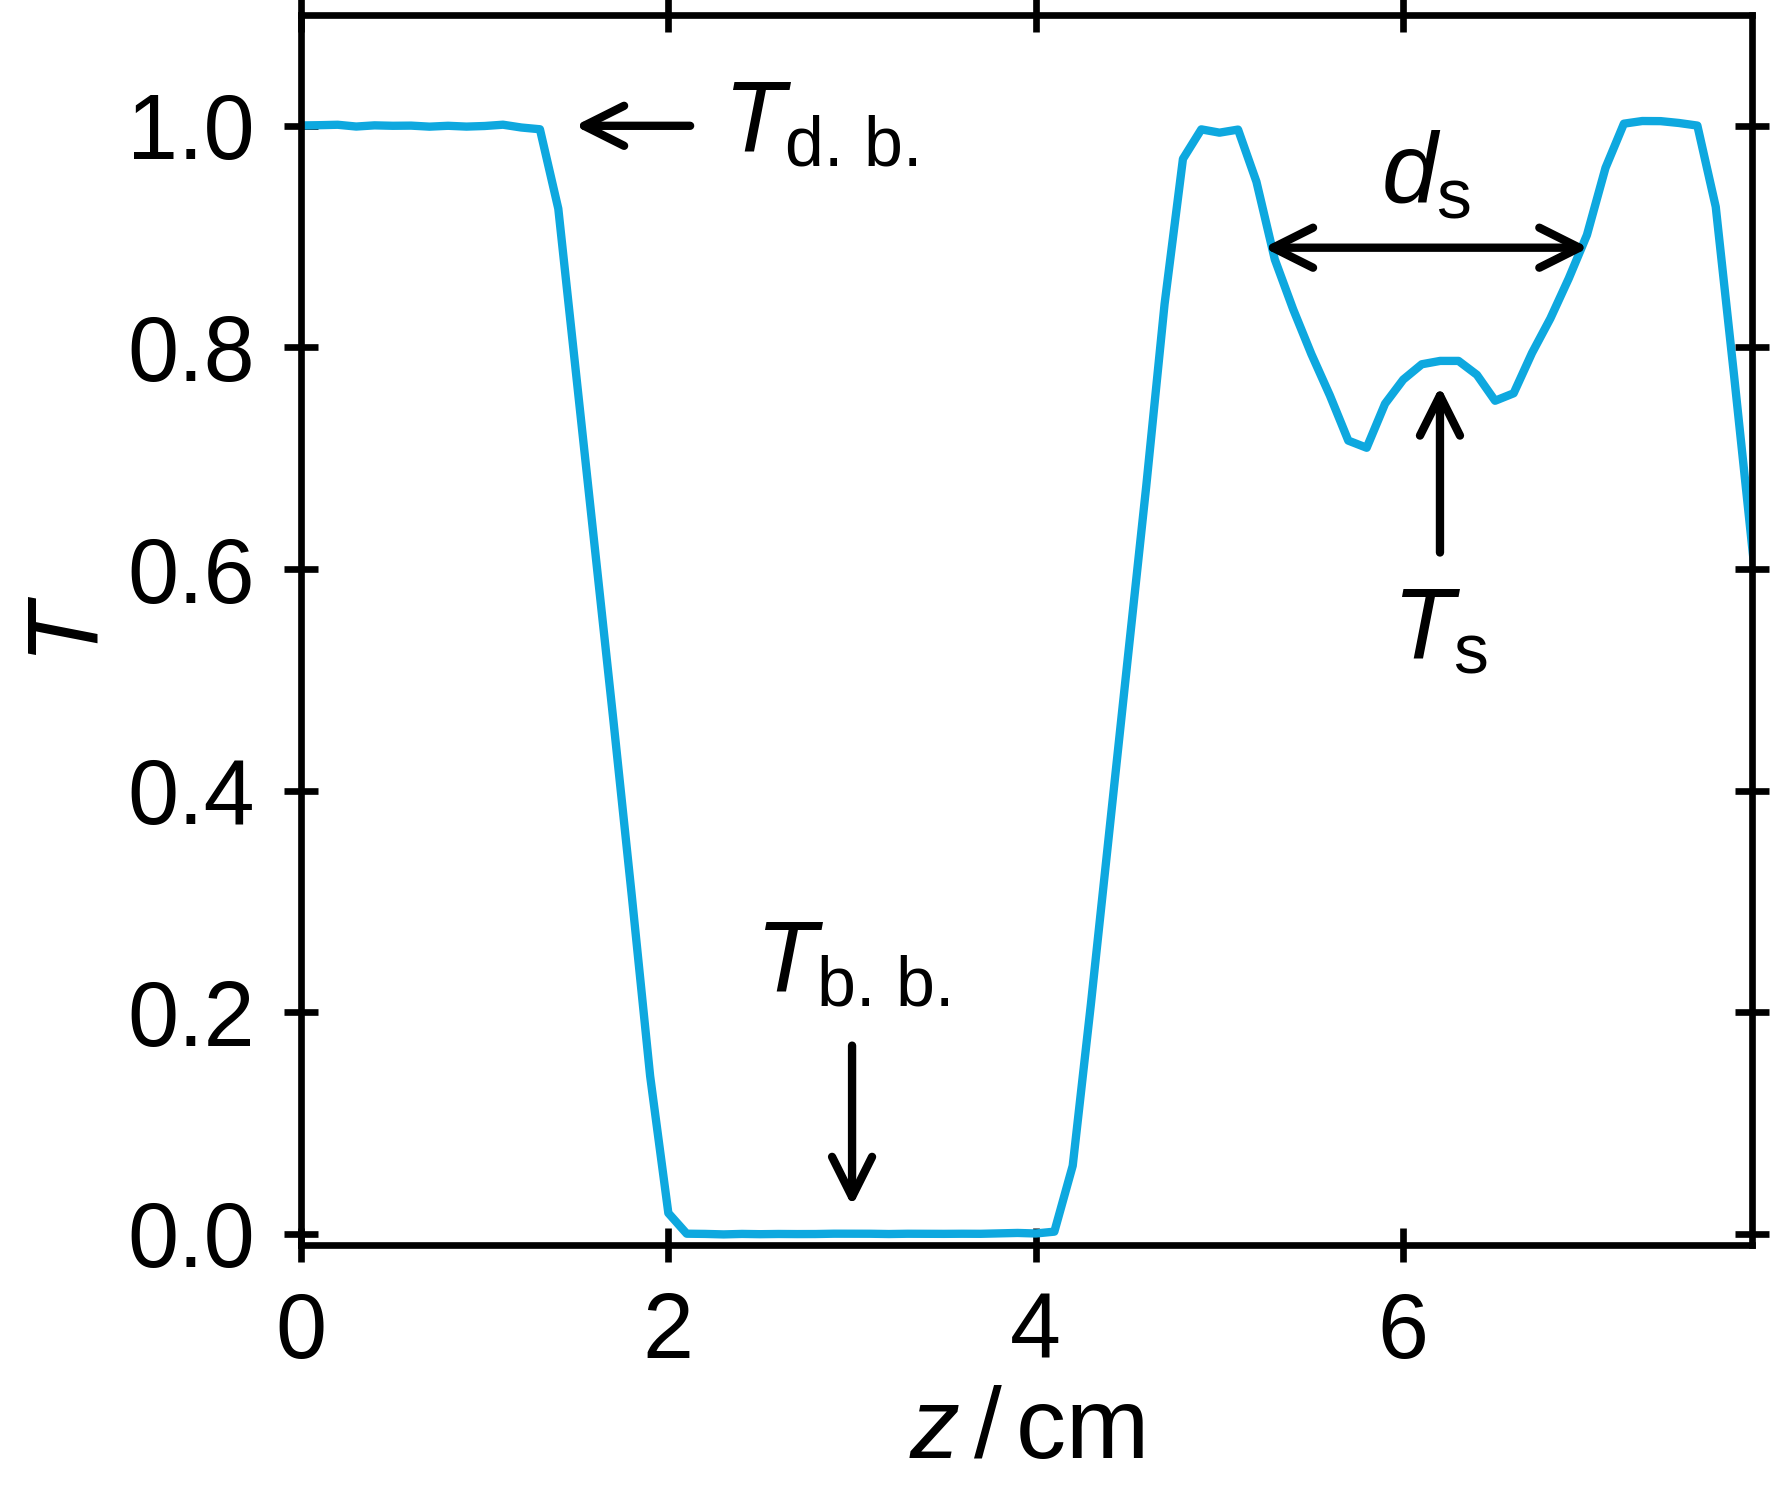
\includegraphics{appendix_methods_SAXS_SampleScan}
      \caption{\label{fig:methods:saxs:fep_scan}Calibration measurement of FEP (left) to determine $I_\mathrm{FEP}^\mathrm{peak}$ and a scan of the vertical transmission of the sample holder (right) from which both the width and the transmission of the sample can be determined to scale the data to absolute units.}
    \end{figure}
    Typically, a profile such as shown in \reffig{fig:methods:saxs:fep_scan} on the right is obtained.
    The scan provides a measure for the intensity of the direct beam, the blocked beam and the profile of the sample.
    By setting the transmission of the direct beam $T_\mathrm{d.\,b.}$ to one and the transmission of the blocked beam to $T_\mathrm{b.\,b.}$ to zero, the value of the scan at the position where the sample is measured provides the transmission of the sample $T_\mathrm{s}$.
    The width of the sample $d_\mathrm{s}$ is estimated as the width read from the sample profile at the half transmission value between the maximum transmission of the sample profile and the determined transmission value at the center.

    After obtaining the azimuthally integrated and scaled intensity in  absolute units, the scattering of the solvent and capillary need to be subtracted from the sample to obtain only the scattering from the nanoparticles.
    As the scattering from the capillary happens to the major part at the glass material and not the inside of the capillary, here the thickness has to be treated differently than in the aforementioned rescaling factor.
    It is assumed that the glass material of all capillaries have approximately the same thickness.
    Then the subtraction of the empty capillary from a sample is straight forward, by performing the rescaling of the sample to it's respective width only after the empty capillary has been subtracted.
    This is done separately for both the sample measurement and the solvent measurement, which are subtracted from each other hereafter.
    To increase the measured range of scattering vector magnitudes $q$, each sample is measured at a relatively small sample-to-detector distance to study the wide $q$ range, and a long sample-to-detector distance to study the low $q$ range.
    Both data sets are merged to a single data set for model calculations.

    All of the laborious steps to determine peak intensities, center positions, distances and transmissions, as well as rescaling and subtraction of the data have been mostly automatized for this work, such that only a minimal amount of input needs to be given to reduce the data live at the experimental site.
    Then focus can be set on modeling the form factor for the obtained scattering curve and discuss the sample structure.
\end{document}